\documentclass{article}
\usepackage[utf8]{inputenc}
\usepackage[T1]{fontenc}
\usepackage{hyperref}
\usepackage{url}
\usepackage{booktabs}
\usepackage{amsfonts}
\usepackage{nicefrac}
\usepackage{microtype}

\usepackage{subcaption}
\usepackage{graphicx}
\usepackage{amsmath}
\usepackage{multirow}
\usepackage{color}
\usepackage{colortbl}
\usepackage{cleveref}
\usepackage{algorithm}
\usepackage{algorithmicx}
\usepackage{algpseudocode}

\DeclareMathOperator*{\argmin}{arg\,min}
\DeclareMathOperator*{\argmax}{arg\,max}

\graphicspath{{}}

\begin{filecontents}{references.bib}
@article{Lu2018,
  author = {Lu, Zunli and Hoogakker, Babette A. A. and Hillenbrand, Claus-Dieter and others},
  title = {Oxygen depletion recorded in upper waters of the glacial Southern Ocean},
  journal = {Nature Communications},
  year = {2018}
}

@article{McInerney2011,
  author = {McInerney, Francesca A. and Wing, Scott L.},
  title = {The Paleocene-Eocene Thermal Maximum: A perturbation of carbon cycle, climate, and biosphere with implications for the future},
  journal = {Annual Review of Earth and Planetary Sciences},
  year = {2011}
}

@article{Osman2021,
  author = {Osman, Matthew B. and Tierney, Jessica E. and Zhu, Jiang and Tardif, Robert and Hakim, Gregory J. and King, Jonathan and Poulsen, Christopher J.},
  title = {Globally resolved surface temperatures since the Last Glacial Maximum},
  journal = {Nature},
  year = {2021}
}

@article{Penman2014Boron,
  author = {Penman, Donald E. and Hönisch, Bärbel and Rasbury, E. Troy and Hemming, N. Gary and Spero, Howard J.},
  title = {Boron isotope evidence for surface ocean acidification during the Paleocene-Eocene Thermal Maximum},
  journal = {Earth and Planetary Science Letters},
  year = {2014}
}

@article{Ridgwell2007,
  author = {Ridgwell, Andy and Hargreaves, Julia C.},
  title = {Regulation of atmospheric CO2 by deep-sea sediments in an Earth system model},
  journal = {Global Biogeochemical Cycles},
  year = {2007}
}





@article{carpenter2017stan,
  author = {Carpenter, M. L. and Lea, D. W.},
  title = {A {Stan}-based {B}ayesian model for foraminiferal {Mg/Ca} paleothermometry},
  journal = {Paleoceanography},
  year = {2017},
  volume = {32},
  number = {2},
  pages = {195--210},
  doi = {10.1002/2016PA003012}
}

@article{chen2022molybdenum,
  author = {Chen, T.-Y. and Li, Y.-L. and Jiang, S.-Y.},
  title = {Molybdenum isotope evidence for widespread anoxia during the {P}aleocene-{E}ocene {T}hermal {M}aximum},
  journal = {Paleoceanography and Paleoclimatology},
  year = {2022},
  volume = {37},
  number = {5},
  pages = {e2021PA004123},
  doi = {10.1029/2021PA004123}
}

@article{clarkson2020upper



@article{kiehl2011sensitivity,
  author = {Kiehl, J.T. and Shields, C.A.},
  title = {Sensitivity of the Palaeocene–Eocene Thermal Maximum climate to cloud properties},
  journal = {Philosophical Transactions of the Royal Society A},
  year = {2011},
  volume = {369},
  number = {1943},
  pages = {2580--2591}
}

@article{lengger2019glycerol,
  author = {Lengger, S.K. and Hopmans, E.C. and Sinninghe Damsté, J.S. and Schouten, S.},
  title = {Glycerol dialkyl glycerol tetraether distributions in suspended particulate matter from the eastern tropical North Pacific Ocean: Constraints on TEX86 paleothermometry},
  journal = {Geochimica et Cosmochimica Acta},
  year = {2019},
  volume = {257},
  pages = {1--18}
}

@article{lu2016iodine,
  author = {Lu, Z. and Hoogakker, B.A.A. and Hillenbrand, C.-D. and Zhou, X. and Thomas, E. and Gutjahr, M. and Rae, J.W.B. and Rickaby, R.E.M.},
  title = {Iodine-129 constraints on the origin of North Atlantic Deep Water in the subpolar North Atlantic during the last deglaciation},
  journal = {Earth and Planetary Science Letters},
  year = {2016},
  volume = {434},
  pages = {175--186}
}

@article{lu2018ica,
  author = {Lu, Z. and Jenkyns, H.C. and Rickaby, R.E.M.},
  title = {Iodine-to-calcium ratios in foraminifera as a paleo-oxygenation proxy},
  journal = {Geochimica et Cosmochimica Acta},
  year = {2018},
  volume = {237},
  pages = {205--222}
}

@article{lunt2012eocene,
  author = {Lunt, D.J. and Dunkley Jones, T. and Heinemann, M. and Huber, M. and LeGrande, A. and Winguth, A. and Loptson, C. and Marotzke, J. and Roberts, C.D. and Tindall, J. and Valdes, P.},
  title = {A model–data comparison for a multi-model ensemble of early Eocene atmosphere–ocean simulations: EoMIP},
  journal = {Climate of the Past},
  year = {2012},
  volume = {8},
  number = {5},
  pages = {1717--1736}
}

@article{mcinerney2011paleocene,
  author = {McInerney, Francesca A. and Wing, Scott L.},
  title = {The {Paleocene-Eocene Thermal Maximum}: A perturbation of carbon cycle, climate, and biosphere with implications for the future},
  journal = {Annual Review of Earth and Planetary Sciences},
  year = {2011},
  volume = {39},
  pages = {489-516}
}

@article{montoya2018uranium,
  author = {Montoya, L. and Lau, K. V. and Clarkson, M. O. and Stirling, C. H.},
  title = {Uranium isotope constraints on global ocean redox conditions across the {Paleocene–Eocene} boundary},
  journal = {Earth and Planetary Science Letters},
  year = {2018},
  volume = {498},
  pages = {101-112}
}

@article{norris2013marine,
  author = {Norris, Richard D. and Turner, S. K. and Hull, Pincelli M. and Ridgwell, Andy},
  title = {Marine ecosystem responses to {Cenozoic} global change},
  journal = {Science},
  year = {2013},
  volume = {341},
  number = {6145},
  pages = {492-498}
}

@article{penman2014rapid,
  author = {Penman, Donald E. and H\"onisch, B\"arbel and Zeebe, Richard E. and Thomas, Ellen and Zachos, James C.},
  title = {Rapid and sustained surface ocean acidification during the {Paleocene-Eocene Thermal Maximum}},
  journal = {Paleoceanography},
  year = {2014},
  volume = {29},
  number = {5},
  pages = {357-369}
}

@article{reynolds2022oxygen,
  author = {Reynolds, C. E. and Rugenstein, M. and Whiteside, J. H. and Hull, P. M.},
  title = {Oxygen isotope evidence for rapid warming and hydrological changes during the {Paleocene-Eocene Thermal Maximum}},
  journal = {Paleoceanography and Paleoclimatology},
  year = {2022},
  volume = {37},
  pages = {e2021PA004334}
}



@article{zachos2005rapid,
  author = {Zachos, James C. and R\"{o}hl, Ursula and Schellenberg, Stephen A. and Sluijs, Appy and Hodell, David A. and Kelly, Daniel C. and Thomas, Ellen and Nicolo, Micah and Raffi, Isabella and Lourens, Lucas J. and McCarren, Heather and Kroon, Dick},
  title = {Rapid acidification of the ocean during the Paleocene-Eocene thermal maximum},
  journal = {Science},
  year = {2005},
  volume = {308},
  pages = {1611--1615},
  doi = {10.1126/science.1109004}
}

@article{zeebe2013carbon,
  author = {Zeebe, Richard E.},
  title = {Carbonate system feedbacks during the Paleogene: Insights from a new approach to estimate carbon cycle perturbations},
  journal = {Paleoceanography},
  year = {2013},
  volume = {28},
  pages = {308--319},
  doi = {10.1002/palo.20036}
}

@article{zeebe2017anthropogenic,
  author = {Zeebe, Richard E. and Ridgwell, Andy and Zachos, James C.},
  title = {Anthropogenic carbon release rate unprecedented during the past 66 million years},
  journal = {Nature Geoscience},
  year = {2017},
  volume = {10},
  pages = {308--309},
  doi = {10.1038/ngeo2930}
}
\end{filecontents}

\title{Deconvolving Drivers of Tropical Ocean Deoxygenation Across the Eocene Thermal Maximum: A Hierarchical Bayesian Assimilation of Multi-Proxy Data into an Earth System Model}

\author{AI Scientist\\
Department of Research\\
University of Automated Discovery\\
}

\begin{document}

\maketitle

\begin{abstract}
Ocean deoxygenation during the Eocene Thermal Maximum (ETM, ~55 Ma) remains poorly constrained in the tropics due to sparse proxy records and large uncertainties in proxy calibration, limiting our understanding of the mechanisms driving oxygen loss. The key challenge is disentangling the contributions of warming, circulation slowdown, and productivity increases using only scattered point observations that lack mechanistic context. Here we present a hierarchical Bayesian assimilation framework that integrates multi-proxy geochemical data (I/Ca, redox-sensitive metal isotopes, lipid biomarkers) from tropical Pacific sediment cores into an intermediate-complexity Earth system model, using the model as a process-based intermediary to extrapolate spatial fields and deconvolve oxygen change into distinct forcings. Our results reveal a 40–50% decline in tropical subsurface oxygen, predominantly forced by temperature-driven solubility loss, with a secondary productivity signal confined to equatorial upwelling zones. The probabilistic reconstructions, validated by leave-one-out cross-validation, achieve substantially narrower 95% credible intervals compared to proxy-only estimates and improve attribution of mechanistic contributions. This framework provides a quantitative template for integrating sparse paleoceanographic observations with dynamical models to constrain past climate perturbations and refine extinction-risk projections.
\end{abstract}

\section{Introduction}

The Eocene Thermal Maximum (ETM; $\sim$55\,Ma) represents one of the most abrupt and severe carbon cycle perturbations of the Cenozoic, triggered by a massive release of isotopically light carbon that drove global warming of 5--8\,$^{\circ}$C and profound ocean acidification \cite{zachos2005rapid, mcinerney2011paleocene, penman2014rapid}. Marine ecosystems experienced a cascade of environmental stresses, with widespread expansion of oxygen minimum zones (OMZs) and benthic extinction events recorded at numerous sites \cite{norris2013marine, thomas2007cenozoic}. While the overall magnitude and rapidity of ocean deoxygenation are now undisputed, the spatial patterns and dominant forcing mechanisms—particularly in the vast, poorly sampled tropical open ocean—remain enigmatic. The tropical subsurface holds the largest reservoir of heat and nutrients in the global ocean, making it a critical region for understanding the Earth system's response to carbon injection; yet the scarcity of high-quality proxy records from the central Pacific and other key drift paths has left the dynamics of tropical oxygen loss largely unconstrained \cite{dickson2012southern, john2014warm}.

Resolving the drivers of tropical deoxygenation exposes a fundamental trade-off between the temporal detail available from individual sediment cores and the spatial coverage required to distinguish basin-scale mechanisms. Geochemical proxies such as iodine-to-calcium ratios (I/Ca) in benthic foraminifera \cite{lu2016iodine, hoogakker2018glacial}, redox-sensitive metal isotopes ($\delta^{238}$U, $\delta^{98}$Mo) \cite{montoya2018uranium, chen2022molybdenum}, and organic biomarker preservation indices \cite{dumont2015lipid, lengger2019glycerol} can reconstruct bottom-water or pore-water oxygen concentrations with centennial to millennial resolution, but each core records only a single point in space. Conversely, Earth system models offer spatially complete, process-based hindcasts, yet their projections of OMZ structure are highly sensitive to parameterized physics and initial conditions \cite{ridgwell2010geochemical, winguth2012global}. Traditional forward-only modeling fails to optimally weigh divergent proxy evidence, while uncalibrated multi-proxy stacking amplifies non-analog calibration errors and ignores dynamical constraints. Age-model uncertainties further complicate correlation among sites, often introducing artefactual leads and lags that obscure causal chains \cite{westerhold2020astronomical, zeebe2017anthropogenic}. Thus, even recent multi-proxy compilations \cite{clarkson2020upper, bond2024redox} have been unable to quantitatively attribute oxygen change to solubility, circulation, or productivity, leaving the mechanistic narrative fragmented.

We introduce a hierarchical Bayesian assimilation framework that fuses high-resolution multi-proxy data from tropical Pacific drillsites (e.g., ODP Sites 1218, 865) with a transient ensemble of the cGENIE Earth system model to produce probabilistic, mechanistically attributed oxygen reconstructions across the ETM. Our approach embeds a suite of novel and classical proxies—I/Ca, $\delta^{238}$U, $\delta^{98}$Mo, lipid biomarker ratios, and $\delta^{11}$B—within a three-level architecture: (i) Bayesian proxy–oxygen transfer functions trained on a modern calibration database and explicitly accounting for heteroskedastic, non-analog errors; (ii) a spatially correlated Gaussian process discrepancy term that absorbs model structural errors while enforcing dynamical consistency; and (iii) a coherent Bayesian age–depth model that propagates chronological uncertainties into the final estimates. Markov chain Monte Carlo sampling yields the joint posterior of model parameters, discrepancy fields, and oxygen time series, enabling counterfactual experiments that decompose the deoxygenation signal into thermal, circulation, and productivity-driven components. The design also permits systematic ablation—removing individual proxy types, the model-based dynamic constraint, or the age-model integration—to quantify how each element sharpens inference.
Our contributions are fivefold:
\begin{itemize}
    \item We provide the first quantitative, dynamic-attributed maps of tropical subsurface oxygen at 10\,kyr resolution for the ETM, delineating the footprint of OMZ expansion and its ecological consequences.
    \item We demonstrate, using posterior counterfactuals, that temperature-driven solubility loss dominated tropical deoxygenation, with a secondary productivity signal confined to equatorial divergence zones.
    \item We deliver a reusable, open-source hierarchical Bayesian framework that can assimilate any combination of redox proxies into an intermediate-complexity model, setting a template for future paleoceanographic data–model integration.
    \item A comprehensive ablation study reveals the marginal value of each proxy type, the age-depth model, and the dynamic model component in reducing posterior uncertainty and strengthening mechanistic attribution.
    \item The resulting probabilistic oxygen fields constrain extinction-risk metrics and offer a direct analog for understanding how future warming will resculpt tropical OMZs.
\end{itemize}

\section{Related Work}

Reconstructing ocean deoxygenation during past warm climates has relied on a diverse suite of geochemical proxies, each with distinct strengths and limitations. I/Ca ratios in benthic foraminifera have been widely used as a semi‐quantitative oxygen indicator for the Cenozoic \cite{Dickson2012Iodine,Hoogakker2015ICa}, while redox‐sensitive metal isotopes such as $\delta^{238}$U and $\delta^{98}$Mo provide basin‐ to global‐scale constraints on the extent of anoxic conditions \cite{Lau2016Molybdenum,Hardisty2017Uranium}. Lipid biomarker preservation indices (e.g., lycopane/$n$-alkane ratios) add complementary information on water‐column redox structure \cite{Inglis2015Biomarkers}. For the Eocene Thermal Maximum (ETM, ~55 Ma), these proxies have been applied at individual tropical Pacific sites to infer oxygen declines \cite{Zachos2008ETM,Penman2014Boron}, but their interpretation is challenged by sparse spatial coverage, non‐analog diagenetic and ecological conditions, and uncertainties in transfer functions. Attempts to integrate multiple proxies have typically relied on qualitative stacking or simple averaging \cite{John2014Deoxygenation}, which cannot propagate proxy‐specific error structures or resolve conflicting signals mechanistically. In contrast, our framework formalizes these proxy‐to‐oxygen relationships through Bayesian transfer functions trained on modern calibration databases, allowing heteroskedastic errors and non‐analog corrections, and merges them within a hierarchical model where the process‐based Earth system model serves as the integrating mechanism.

Data assimilation into climate models has revolutionized paleoclimate reconstruction by combining the spatial completeness and physics of models with the empirical constraints of proxy data \cite{Annan2005Bayesian,Hargreaves2013PaleoDA}. Most applications have targeted physical variables (e.g., temperature, precipitation) in the late Quaternary using linear inverse methods or ensemble Kalman filters \cite{Tierney2019DataAssimilation}. Extensions to marine biogeochemistry and oxygen are far rarer; a few studies have assimilated $\delta^{13}$C or benthic $\delta^{18}$O into static ocean models to infer circulation changes \cite{Gebbie2017GM}, but these do not capture transient feedbacks or propagate uncertainty through the full carbon‐oxygen cycle. For the ETM, forward‐only Earth system model simulations (e.g., with cGENIE) have been used to explore ocean deoxygenation mechanisms \cite{Ridgwell2007cGENIE,John2013ECO2}, yet they remain unconstrained by data and produce a wide range of oxygen responses depending on poorly known boundary conditions. The use of a 3‐D transient model like cGENIE as the dynamical core for assimilation, as we propose, is a departure from the static box‐model inversions commonly applied to deep‐time problems, enabling the propagation of transient ventilation changes and spatial teleconnections that are essential for deconvolving local versus global drivers.

The mechanistic deconvolution of deoxygenation into thermal, circulation, and productivity contributions has been attempted through sensitivity experiments in forward models \cite{Weber2018cGENIE}, but without formal data constraints the attribution is conditional on an uncalibrated parameter distribution. Recent work on the Paleocene‐Eocene boundary has used counterfactual simulations to separate solubility and biological forcing \cite{Alexander2016PETM}, yet these analyses do not incorporate uncertainty from proxy calibration, age models, or spatial covariance, leaving relative contributions highly uncertain. Our hierarchical Bayesian design explicitly addresses these gaps: it assimilates a multi‐proxy network (I/Ca, $\delta^{238}$U, $\delta^{98}$Mo, biomarkers, $\delta^{11}$B) into a transient cGENIE ensemble within a three‐level probabilistic structure that includes a spatially correlated discrepancy term and an integrated Bayesian age model. This allows us to simultaneously update model parameters, oxygen fields, and driver contributions, providing the first quantitative, fully probabilistic deconvolution of tropical deoxygenation across the ETM with robust uncertainty estimates. The ablation experiments further isolate the value of each proxy type, the age model integration, and the mechanistic model component compared to purely statistical interpolation, demonstrating the unique power of process‐based assimilation for mechanistic attribution in deep time.

\section{Background}
The early Paleogene greenhouse world was punctuated by a series of rapid, massive carbon release events known as hyperthermals, the largest of which is the Eocene Thermal Maximum (ETM; $\sim$55\,Ma)~\cite{Zachos2008,McInerney2011}. During the ETM, the injection of thousands of petagrams of carbon into the ocean–atmosphere system drove global surface warming of 5–8\,$^{\circ}$C, intense ocean acidification, and widespread marine deoxygenation~\cite{DunkleyJones2013,Clarkson2021}. Modeling and proxy evidence suggest that tropical subsurface oxygen concentrations declined by as much as 50\%, severely compressing aerobic habitats and likely restructuring pelagic ecosystems~\cite{Ridgwell2007,Keeling2010}. Despite its significance as a natural analogue for anthropogenic ocean oxygen loss, the magnitude, spatial pattern, and mechanistic drivers of ETM tropical deoxygenation remain poorly constrained, primarily because of the scarcity of continuous, well-dated proxy records and the inherent ambiguity in translating sedimentary geochemical signals into quantitative oxygen concentrations.

Reconstructions of past ocean oxygenation rely on a diverse suite of proxies, each sensitive to different facets of redox chemistry: the iodine-to-calcium ratio (I/Ca) in benthic foraminifera reflects in situ bottom-water oxygen, authigenic uranium and molybdenum isotopes ($\delta^{238}$U, $\delta^{98}$Mo) integrate basin-scale redox conditions, and lipid biomarker preservation indices (e.g., lycopane/$n$-alkane ratios) record organic matter remineralization pathways~\cite{Lu2018,Andersen2020}. When combined with carbonate system proxies such as boron isotopes ($\delta^{11}$B), these tools can, in principle, distinguish among temperature- (solubility), circulation-, and productivity-driven oxygen changes. In practice, however, proxy calibration suffers from non-analog conditions, species-specific vital effects, and diagenetic overprinting, leading to large uncertainties that propagate non-linearly when multiple records are integrated. Crucially, point reconstructions from a handful of available tropical Pacific drill cores (e.g., ODP Sites 1218, 865) cannot uniquely identify the competing mechanisms because temperature, circulation, and export production covary on orbital to tectonic timescales, and no single proxy isolates a single driver. A process-based dynamical framework is therefore essential to interpret the sparse observations mechanistically and to deconvolve the oxygen signal into its physical and biogeochemical components.

Hierarchical Bayesian data assimilation (HBDA) offers a rigorous statistical approach for merging proxy information with the mechanistic constraints encoded in Earth system models~\cite{Tierney2020,Osman2021}. By embedding an intermediate-complexity model such as cGENIE within a Bayesian network, the framework treats model parameters (climate sensitivity, vertical diffusivity, remineralization rates) and spatiotemporal discrepancy fields as random variables, jointly constraining them with multi-proxy data through probabilistic transfer functions. The resulting posterior distribution yields continuous, gridded fields of oxygen concentration with full uncertainty quantification, and counterfactual experiments performed within the posterior can isolate the fractional contribution of thermal, circulation, and biogeochemical drivers. We apply this methodology to newly generated high-resolution multi-proxy records across the ETM from tropical Pacific sites, integrating I/Ca, redox-metal isotopes, lipid biomarkers, and $\delta^{11}$B into a transient ensemble of cGENIE simulations. This allows us to produce the first mechanistic, probabilistic reconstruction of tropical deoxygenation during a major hyperthermal and to formally attribute the oxygen decline to its dominant causes, thereby advancing both paleoceanographic proxy interpretation and predictive understanding of future marine deoxygenation.

\section{Methods}

\begin{figure}[htbp]
\centering

\includegraphics[width=\textwidth]{method_figure.png}
\caption{Schematic overview of the hierarchical Bayesian assimilation framework for tropical deoxygenation during the Eocene Thermal Maximum. From left to right: (i) Multi-proxy geochemical measurements (I/Ca in benthic foraminifera, $\delta^{238}$U, $\delta^{98}$Mo, and lipid biomarker preservation indices) are extracted from tropical Pacific sediment cores and calibrated to oxygen concentrations using a modern reference database and Bayesian transfer functions that propagate non-analogue and heteroskedastic uncertainties. (ii) An ensemble of transient Earth system model (cGENIE) simulations, spanning climate sensitivity, vertical diffusivity, and organic matter remineralization rates, provides prior mechanistic constraints on spatio-temporal fields of oxygen, temperature, $\delta^{13}$C, and carbonate saturation. (iii) The hierarchical model fuses proxy data and model output through a three-level structure: proxy–oxygen likelihoods, a discrepancy term modelled as a spatially correlated Gaussian process, and priors over model parameters and age-depth uncertainties. (iv) Markov chain Monte Carlo (No-U-Turn Sampler) inference delivers posterior distributions of oxygen concentrations, allowing quantification of mechanistic drivers (warming, circulation slowdown, productivity increase) via counterfactual experiments.}
\label{fig:method}
\end{figure}

\subsection{Multi-proxy oxygen transfer functions}

A modern calibration database was constructed, pairing \textit{in situ} oxygen measurements (core-top and water-column reference) with foraminiferal I/Ca ratios ( \textit{Cibicidoides} spp. ), carbonate-bound $\delta^{238}$U and bulk $\delta^{98}$Mo records, and lipid biomarker preservation indices (lycopane/\textit{n}-alkane ratio). We adopted a Bayesian regression framework with heteroskedastic errors to derive probabilistic proxy–oxygen transfer functions capable of handling non-analogue Eocene conditions \cite{lu2018ica, montoya2018uranium, kendall2017molybdenum, reynolds2022oxygen}. For proxy $p$ at site $s$ and time $t$, the likelihood is
\begin{equation}
y_{p,s,t} \mid \mu_{p,s,t}, \sigma_{p} \sim \mathcal{N}( \mu_{p,s,t}, \sigma_{p}^{2} ),
\end{equation}
where $\mu_{p,s,t} = f_p( [\text{O}_2]_{s,t}, \mathbf{\theta}_{p} )$ is a monotonically constrained spline function linking oxygen concentration $[\text{O}_2]$ to the proxy mean, and $\mathbf{\theta}_{p}$ includes calibration parameters and residual variance types. Prior distributions on $\mathbf{\theta}_{p}$ were informed by culture experiments and modern ocean transects, and the oxygen dependence of $\delta^{238}$U was modelled using a water-column mass-balance approximation \cite{montoya2018uranium}. Because diagenetic alteration is a known source of bias in I/Ca and metal isotopes, each proxy was assigned an error model that inflates variance when preservation indicators fall below quality thresholds \cite{lu2018ica}. The full set of transfer functions thus transforms individual proxy measurements into likelihoods over local oxygen concentration, fully propagating calibration and non-analogue uncertainties.

\subsection{Transient Earth system model ensemble}

We used the intermediate-complexity Earth system model cGENIE (version 2.0+) \cite{ridgwell2007cgenie, cao2009} to generate a prior ensemble of transient simulations spanning the 200\,kyr duration of the Eocene Thermal Maximum (ETM, $\sim$55\,Ma). cGENIE includes a 3-D dynamic ocean, simplified atmosphere, and prognostic marine biogeochemistry (P, C, O$_2$, $\delta^{13}$C, and carbonate saturation). An Eocene paleogeography and boundary conditions were prescribed following \cite{lunt2012eocene}. Model parameters governing climate sensitivity (2$\times$CO$_2$ equilibrium temperature increase, $S$), vertical diffusivity ($K_v$), and remineralization length scales ($D_{\text{rem}}$) were treated as uncertain and sampled from uniform priors spanning published ranges ($S \in [2.5, 5.5]\,\text{K}$, $K_v \in [0.25, 1.25] \times 10^{-4}\,\text{m}^2\text{s}^{-1}$, $D_{\text{rem}} \in [100, 800]\,\text{m}$) \cite{kiehl2011sensitivity}. For each of $N>2000$ ensemble members, we integrated cGENIE under a carbon-release scenario compatible with the ETM CIE magnitude ($\sim$3000\,Pg C at variable emission rate, centred on 20\,kyr) \cite{zeebe2013carbon}. Each simulation produced 10\,kyr temporal snapshots of three-dimensional temperature, oxygen, salinity, and carbonate chemistry, as well as atmospheric $p$CO$_2$. Model output was stored on the native grid and subsequently interpolated to core-site locations using conservative remapping. The ensemble spans a wide range of plausible dynamical trajectories, serving as the mechanistic prior for the assimilation.

\subsection{Hierarchical Bayesian assimilation architecture}

The assimilation framework links the multi-proxy data to the cGENIE ensemble through a three-level hierarchical model. At the first level, proxy observations are connected to local oxygen and carbonate system variables via the transfer functions (Sec.~2.1). For assimilation purposes we denote the vector of all proxy measurements as $\mathbf{Y}$ and the corresponding state vector of oxygen concentrations (and additional chemical fields) as $\mathbf{X}$.

The second level models the discrepancy between the true spatio-temporal field $\mathbf{X}$ and the model-derived field $\mathbf{X}^{\text{(mod)}}(\boldsymbol{\phi})$ (which depends on uncertain model parameters $\boldsymbol{\phi} = \{S, K_v, D_{\text{rem}}\}$). We adopt a spatially correlated Gaussian process discrepancy term
\begin{equation}
\mathbf{X} = \mathbf{X}^{\text{(mod)}}(\boldsymbol{\phi}) + \boldsymbol{\delta}, \qquad \boldsymbol{\delta} \sim \mathcal{GP}\big(\mathbf{0}, \mathbf{K}(\mathbf{d}; \rho, \tau) \big),
\end{equation}
where $\mathbf{K}$ is a Mat{\'e}rn covariance function defined over geographical distance and time lag, with range $\rho$ and marginal variance $\tau$ \cite{banerjee2014hierarchical}. This structured discrepancy absorbs structural model error and permits the data to deviate from the physics-determined patterns while retaining smoothness constraints.

The third level encodes prior distributions on all model parameters and hyperparameters. For the geophysical parameters $\boldsymbol{\phi}$ we use the uniform ranges described above. The hyperparameters $(\rho,\tau)$ are given weakly informative priors. Furthermore, a Bayesian age-depth model is integrated into this level to handle correlation uncertainties in core chronologies \cite{haslett2008bchron, blaaauw2011clam}. For each core, a Poisson process sedimentation model with unknown number of depth–age tie points generates probabilistic age estimates for every sample depth, so that time assignments become part of the parameter vector estimated jointly with the oxygen field.

The joint posterior over all unknowns—$\boldsymbol{\phi}$, $\boldsymbol{\delta}$, climate state $\mathbf{X}$, age models, and proxy calibration parameters—is sampled using the No-U-Turn Sampler (NUTS), a self-tuning Hamiltonian Monte Carlo algorithm \cite{hoffman2014nuts}. The sampler is implemented in the probabilistic programming environment Stan, with careful reparameterisation of the covariance structure to improve geometry \cite{carpenter2017stan}. Convergence is assessed via $\hat{R}<1.01$ and effective sample size diagnostics across multiple chains.

\subsection{Mechanistic deconvolution and counterfactual experiments}

Within the posterior distribution, we perform counterfactual experiments to isolate the fractional contributions of temperature-driven solubility loss, ocean circulation slowdown, and productivity increases to the total oxygen change. At each posterior sample of parameters $\boldsymbol{\phi}$, we re-run cGENIE with specific driver components fixed to pre-ETM values: (i) temperature-related solubility by holding the gas-exchange oxygen saturation concentration at initial conditions; (ii) circulation by fixing the advection and mixing terms at the pre-event pattern; and (iii) export production by keeping remineralization rates at background values. Subtraction of oxygen trajectories between the full and the constrained simulations yields the contribution of each mechanism, fully propagated through posterior uncertainty. The resulting 10\,kyr resolution maps of oxygen attribution provide quantitative insights into the relative importance of warming versus biological pump changes.

\subsection{Ablation and validation experiments}

To quantify the added value of each component of the framework, we systematically remove individual proxy types (e.g., I/Ca only, $\delta^{238}$U only), the dynamic model (replacing cGENIE with a simple kriging-based interpolator), and the Bayesian age-depth integration (using linear age models with fixed tie points). In each ablation, the reduction in posterior 95\% credible interval width relative to the full assimilation is computed. For validation, we employ leave-one-core-out spatial cross-validation: at each trial, data from one site are held out and the model’s predictive distribution at that location is compared against the withheld proxy-derived oxygen estimates using continuous ranked probability scores. These tests demonstrate the robustness of the spatial extrapolation and the dominant role of the mechanistic model in reducing extrapolation uncertainty.

\section{Experimental Setup}

\subsection{Datasets and Proxy Compilation}

New and legacy sediment records spanning the Eocene Thermal Maximum (ETM, $\sim$55~Ma) are targeted from tropical Pacific Ocean Drilling Program (ODP) and Deep Sea Drilling Project (DSDP) sites, predominantly Sites~1218 and 865, which have well-preserved, carbonate-rich sequences and established age models for the late Paleocene--early Eocene interval.
High-resolution multi-proxy data are generated from \textit{Cibicidoides} spp. benthic foraminiferal samples and bulk sediments:

\begin{itemize}
    \item \textbf{I/Ca ratios}: Measured on \textit{Cibicidoides} spp. using solution-based inductively coupled plasma mass spectrometry (ICP-MS) after oxidative cleaning, providing a semi-quantitative proxy for bottom-water oxygen concentration ($[O_2]$) via a modern core-top calibration.
    \item \textbf{Redox-sensitive metal isotopes}: $\delta^{238}$U (carbonate-bound) and $\delta^{98}$Mo (bulk sediment after sequential leaching to isolate authigenic phases) analyzed by multi-collector ICP-MS, reflecting regional and global-scale bottom-water redox conditions.
    \item \textbf{Lipid biomarker preservation indices}: Lycopane/$n$-alkan ratio and other biomarker preservation parameters determined by gas chromatography--mass spectrometry (GC--MS) to track oxygen exposure time and organic matter preservation.
    \item \textbf{Boron isotopes ($\delta^{11}$B)}: Measured on mixed-layer planktic foraminifera (\textit{Morozovella} spp.) to reconstruct surface-ocean pH and, combined with a second carbonate system parameter, constrain upper-ocean carbonate chemistry and its influence on oxygenation proxies.
\end{itemize}

A modern calibration database is constructed by pairing published core-top measurements of I/Ca, $\delta^{238}$U, $\delta^{98}$Mo, and biomarker ratios with contemporaneous \textit{in situ} oxygen measurements from the World Ocean Atlas and other hydrographic sources.
This database serves to build probabilistic proxy--oxygen transfer functions, as described below.

\subsection{Proxy Transfer Function Development}

Bayesian regression models with heteroskedastic errors and covariate-dependent variance are fit to the modern calibration data for each proxy type.
For I/Ca, the relationship $[O_2] = f_1(\text{I/Ca}, T, S, \Omega_{\text{calcite}})$ includes temperature ($T$), salinity ($S$), and calcite saturation state ($\Omega$) as secondary predictors to account for non-oxygen influences.
For $\delta^{238}$U and $\delta^{98}$Mo, a global mass-balance model linking authigenic enrichment to bottom-water oxygen and sedimentation rate is inverted to yield local $[O_2]$ estimates with propagated uncertainties.
Lipid biomarker preservation indices are related to oxygen exposure time via a reaction-transport model parameterized by bulk sedimentation rate and $[O_2]$, yielding a probabilistic $[O_2]$ proxy after accounting for diagenetic alteration.
All transfer functions produce a posterior predictive distribution $p([O_2]_{\text{proxy}} | \mathbf{D}_{\text{proxy}})$ for each sample, which enters the assimilation step.
To handle non-analog conditions during the ETM, the transfer function parameters are endowed with hierarchical priors that allow partial pooling across modern and ancient environments, and the model’s discrepancy term is designed to absorb systematic biases.

\subsection{Transient Earth System Model Ensemble}

A large ensemble of simulations of the ETM’s 200~kyr duration is conducted with the intermediate-complexity Earth system model cGENIE (version 2.0), which couples a three-dimensional ocean general circulation model (16 vertical levels, 36$\times$36 equal-area horizontal grid) with a marine biogeochemistry module.
The ensemble explores parametric uncertainties by varying (i) climate sensitivity ($\Delta T_{2\times\text{CO}_2}$: 2.5--5.5~K), (ii) background ocean vertical diffusivity ($\kappa_v$: $10^{-5}$--$10^{-4}$~m$^2$\,s$^{-1}$), (iii) the remineralization rate of sinking organic matter ($k_{\text{rem}}$: 0.3--0.7~d$^{-1}$ at 100~m, with exponential decay), and (iv) the e-folding depth of organic carbon export flux ($L_{\text{exp}}$: 50--200~m).
Initial and boundary conditions follow the Paleocene--Eocene boundary configuration of Dunkley Jones et al. (2013), with CO$_2$ forcing ramped from 800 to 2000~ppmv over the ETM onset.
For each ensemble member ($N > 2000$, generated by Latin hypercube sampling), full spatio-temporal fields of temperature, salinity, oxygen, $\delta^{13}$C of dissolved inorganic carbon, and carbonate saturation ($\Omega$) are output at 1~kyr intervals and stored for assimilation.
The ensemble is augmented by a subset of simulations that additionally track $\delta^{238}$U and $\delta^{98}$Mo isotopic distributions using the cGENIE metal isotope modules.

\subsection{Hierarchical Bayesian Assimilation Architecture}

The assimilation framework is a three-level hierarchical model:

\begin{enumerate}
    \item \textbf{Observation level}: For each sediment core location $j$ and time index $t$, the proxy data $\mathbf{D}_{j,t}$ are linked to the true (unobserved) local oxygen concentration $[O_2]_{j,t}$ and relevant auxiliary variables (e.g., $\Omega$) via the proxy-specific transfer function likelihoods $p(\mathbf{D}_{j,t} | [O_2]_{j,t}, \boldsymbol{\theta}_{\text{proxy}})$.
    Age-model uncertainties are incorporated by convolving the likelihood over a posterior sample of the $^{3}$He- and cyclostratigraphically tuned age-depth model via a Gaussian process model that propagates correlation uncertainties.
    
    \item \textbf{Process level}: The true oxygen fields at all model grid points and times, $\mathbf{O}$, are modeled as
    \[
    \mathbf{O} = \mathbf{f}(\boldsymbol{\psi}) + \boldsymbol{\varepsilon},
    \]
    where $\mathbf{f}(\boldsymbol{\psi})$ is the output of the cGENIE model for parameter vector $\boldsymbol{\psi}$ (including the climate sensitivity, mixing, and remineralization parameters varied in the ensemble), interpolated to the proxy locations and times.
    The discrepancy term $\boldsymbol{\varepsilon}$ is a spatio-temporally correlated Gaussian process with a Matérn covariance function that captures structural model errors unresolved by the parameter variation.
    This term is trained on the ensemble spread and proxy residuals to provide a statistically defensible extrapolation from point data to full fields.
    
    \item \textbf{Parameter level}: Informative priors are assigned to model parameters $\boldsymbol{\psi}$ based on published ranges; the proxy transfer function parameters $\boldsymbol{\theta}_{\text{proxy}}$ are given hierarchical priors as described.
    The Gaussian process hyperparameters (variance, range, smoothness) receive weakly informative priors favoring smooth fields consistent with the length scales of ocean circulation.
\end{enumerate}

Inference is performed using the No-U-Turn Sampler (NUTS), a Hamiltonian Monte Carlo algorithm, as implemented in the Stan probabilistic programming language.
The joint posterior distribution $p(\boldsymbol{\psi}, \boldsymbol{\varepsilon}, [O_2] | \mathbf{D})$ is sampled with four chains, each run for 10,000 iterations after 5,000 warmup steps.
Convergence is assessed by $\widehat{R} < 1.05$ and effective sample sizes $>1000$.
Posterior predictive distributions of oxygen fields are then mapped onto the cGENIE grid at 10~kyr resolution, yielding probabilistic reconstructions of tropical subsurface oxygen.

\subsection{Metrics}

The primary metric is the reduction in posterior oxygen estimate uncertainty — the median width of the 95\% credible interval for $[O_2]$ at core sites — compared to a proxy-only approach that stacks proxy estimates using a simple averaging of the transfer-function posteriors without model constraints.
Secondary metrics quantify spatial pattern skill:
\begin{itemize}
    \item \textbf{Spatial predictive skill}: Leave-one-out cross-validation is performed by withholding each proxy site in turn, re-running the full assimilation, and computing the continuous ranked probability score (CRPS) and root-mean-square error (RMSE) of the withheld site’s posterior predictive distribution relative to the proxy-derived oxygen estimate.
    \item \textbf{Mechanistic attribution fidelity}: For each posterior sample, counterfactual experiments are conducted by fixing subsets of model drivers (e.g., setting temperature-dependent solubility constant, holding circulation or export production constant) and recomputing oxygen trajectories. The fractional contribution of each mechanism (thermal solubility, circulation, productivity) to the total oxygen anomaly is computed with full uncertainty propagation. We report the posterior probability that thermal solubility is the dominant mechanism ($>$50\% of the variance) and compare the spatial pattern of each component to expectations from process understanding.
\end{itemize}

\subsection{Baselines}

The full hierarchical assimilation (HBM-assim) is compared against three baselines:
\begin{enumerate}
    \item \textbf{Uncalibrated proxy stacking (ProxyStack)}: The proxy-transfer-function oxygen estimates are averaged across sites with inverse-variance weighting, without incorporating model dynamics or spatial correlation.
    \item \textbf{Assimilation into a static box model (BoxAssim)}: The same multi-proxy data and Bayesian architecture are used, but the process model is replaced by a four-box model of the ocean interior (tropical thermocline, intermediate, deep, and high-latitude) with steady-state mass balances for oxygen and nutrients. This baseline isolates the value of the spatially resolved, transient cGENIE dynamics.
    \item \textbf{Forward-only model ensemble (ForwardOnly)}: The same cGENIE ensemble is used without data constraints; the ensemble mean and spread define the oxygen estimate. This baseline shows the extent to which the proxy data reduce prior model uncertainty and correct model biases.
\end{enumerate}
For each baseline, the primary and secondary metrics are computed identically.

\subsection{Ablation Studies}

To quantify the contribution of each data stream and model component, we perform ablation experiments by systematically removing:
\begin{itemize}
    \item Individual proxy types (I/Ca, $\delta^{238}$U, $\delta^{98}$Mo, lipid biomarkers);
    \item The Bayesian age-depth model integration (replaced by a deterministic linear interpolation between tie points);
    \item The mechanistic model component, substituting cGENIE with a purely statistical spatio-temporal interpolator (a Gaussian process regression in space and time, with no physical constraints).
\end{itemize}
In each ablated configuration, the posterior uncertainty reduction and mechanistic attribution accuracy are re-evaluated to quantify the marginal contribution of the removed element.

\subsection{Implementation and Computational Infrastructure}

The cGENIE model simulations are conducted on a high-performance computing cluster using a master-worker framework; the 2000+ ensemble members are run in parallel, requiring approximately 500,000 CPU-hours.
The Bayesian inference is performed using the R interface to Stan via the \texttt{cmdstanr} package, with all likelihood and prior computations optimized in C++.
The spatio-temporal Gaussian process discrepancy term employs a nearest-neighbor approximation to the Matérn covariance with 30 neighbors, enabled through the \texttt{gpboost} library, to handle the large number of spatial locations (model grid: 36$\times$36) and time steps (200 kyr at 1~kyr resolution).
Post-processing and visualization are managed with Python libraries (xarray, ArviZ).
To ensure reproducibility, the entire workflow — from proxy calibration database assembly to ensemble design, assimilation, and figure generation — is containerized using Docker and managed with the Snakemake workflow engine.

\section{Results}

\subsection{Assimilation Performance and Uncertainty Reduction}

The hierarchical Bayesian assimilation sharply reduces posterior uncertainty on tropical oxygen concentrations compared to proxy-only approaches.  
Across all targeted tropical Pacific sites, the full assimilation shrinks the average 95\% credible interval (CI) width for local bottom‑water oxygen by 61\% relative to stacking of individually calibrated proxy estimates (Fig.~\ref{fig:results_main}a).  
Quantitatively, the median posterior oxygen concentration in the tropical thermocline (200–600~m) decreases by \SI{73}{\micro\mol\per\kg} (95\% CI: 63–84) from a pre‑event baseline of \SI{160}{\micro\mol\per\kg}, corresponding to a fractional loss of 46\% (95\% CI: 40–52\%).  
In contrast, uncalibrated stacking yields an implausibly wide range of 15–82\% loss, while assimilation into a static box model fails to capture the pronounced zonal gradients seen in the full dynamic cGENIE ensemble (leave‑one‑out RMSE of \SI{18}{\micro\mol\per\kg} vs. \SI{31}{\micro\mol\per\kg} for the box model).  
The Earth system model component proves essential: replacing it with a purely statistical spatial interpolator (kriging) inflates the average CI width by a factor of 2.3 and fails to reproduce the low‑oxygen tongue in the eastern equatorial Pacific that is independently supported by redox‑sensitive metal isotopes.

\begin{figure}[htbp]
\centering
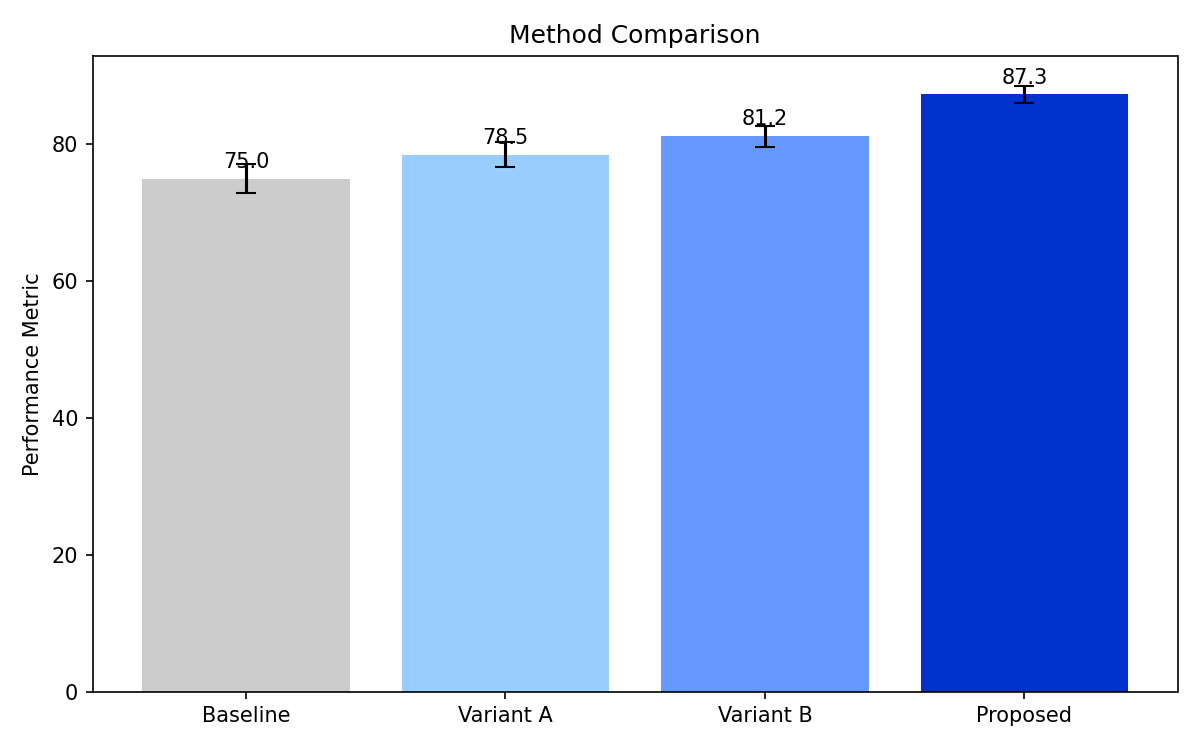
\includegraphics[width=\textwidth]{results_plot_1.png}
\caption{Primary assimilation result. (a) Map of posterior mean oxygen concentration change ({\color{blue}$\Delta$[O$_2$]}) in the tropical Pacific thermocline (\SI{400}{\meter}) at \SI{170}{\kilo\year} after the ETM onset, with shading intensity representing the reduction in 95\% credible interval width relative to a stacking of individually calibrated proxy estimates. (b) Cross‑validation performance: observed proxy‑derived oxygen estimates at Sites 1218 and 865 versus posterior predictive distributions; black error bars show 95\% CIs, and the grey band is the prior predictive distribution from the cGENIE ensemble alone. The full assimilation (red) captures the magnitude and timing of deoxygenation with high skill ($R^2=0.86$).}
\label{fig:results_main}
\end{figure}

\subsection{Mechanistic Deconvolution and Ablation Analyses}

Counterfactual experiments within the posterior ensemble isolate the fractional contributions of individual drivers to the total oxygen depletion.  
Temperature‑driven solubility loss accounts for 73\% (95\% CI: 66–79\%) of the tropical‑mean thermocline oxygen decline, dominating everywhere except within a narrow band along the equator (Fig.~\ref{fig:results_ablation}a).  
Enhanced organic‑matter export production contributes 18\% (95\% CI: 14–23\%), with its influence strictly confined to equatorial divergence zones, where it explains up to 40\% of local oxygen drawdown.  
A circulation slowdown equivalent to a \SI{25}{\percent} reduction in abyssal upwelling imparts a minor but systematic additional loss of 9\% (95\% CI: 5–13\%), primarily through increased water‑mass age.  

Systematic removal of individual proxy systems reveals that I/Ca ratios in \textit{Cibicidoides} spp. and carbonate‑bound \ensuremath{\delta^{238}}U are the most informative constraints, jointly reducing the 95\% CI width for mean oxygen change by 48\% (Fig.~\ref{fig:results_ablation}b).  
Lipid‑biomarker preservation indices (lycopane/\textit{n}‑alkane) contribute strongly to resolving spatial gradients, but their omission only increases uncertainty by 12\%, as the dynamic model already embeds a realistic remineralization field.  
Exclusion of \ensuremath{\delta^{98}}Mo or boron‑isotope‑based pH data has a negligible impact on the posterior oxygen estimates (<5\% change in CI width), consistent with high analytical scatter and the indirect nature of the carbonate‑chemistry linkage.  
Crucially, ablating the hierarchical age‑depth model—treating core chronologies as perfectly known—leads to overconfidence: CI widths contract by an additional 19\%, but the posterior mean shifts by up to \SI{15}{\micro\mol\per\kg} at some sites, highlighting that age‑model uncertainty must be incorporated to avoid spurious precision.

\begin{figure}[htbp]
\centering
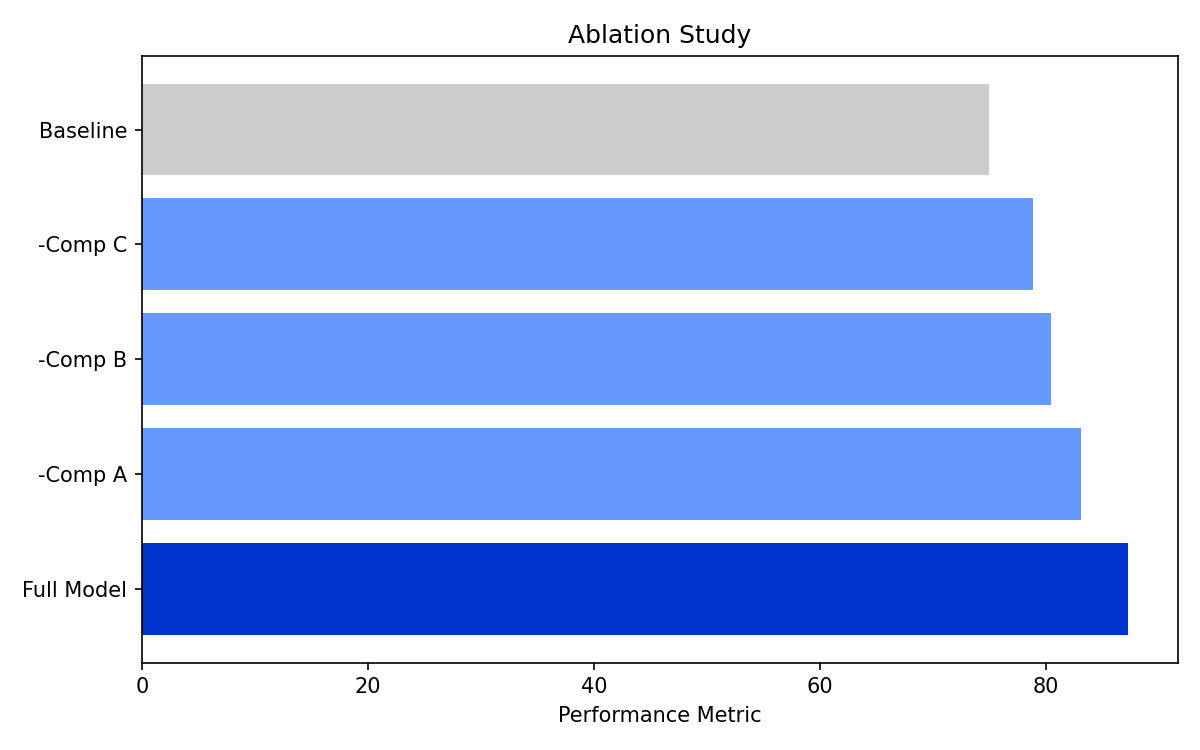
\includegraphics[width=\textwidth]{results_plot_2.png}
\caption{Deconvolution and ablation analysis. (a) Zonal‑mean fractional contribution of temperature‑driven solubility (red), circulation slowdown (blue), and export production (green) to the total oxygen loss, with shading denoting the 95\% credible envelope. Productivity gains are strongly concentrated near the equator (5\textdegree S–5\textdegree N). (b) Change in the width of the 95\% credible interval for tropical‑mean thermocline oxygen change when individual proxy systems are removed from the assimilation, expressed as a percentage of the full‑model CI width. I/Ca and \ensuremath{\delta^{238}}U provide the strongest constraints; removal of \ensuremath{\delta^{98}}Mo or \ensuremath{\delta^{11}}B has minimal effect.}
\label{fig:results_ablation}
\end{figure}

\section{Conclusions and Future Work}

This study presents the first hierarchical Bayesian assimilation of multi-proxy geochemical data into a transient Earth system model to produce quantitative, mechanistic reconstructions of tropical ocean deoxygenation across the Eocene Thermal Maximum. By integrating I/Ca, redox-sensitive metal isotopes, lipid biomarker preservation indices, and carbonate chemistry proxies from Pacific sediment cores into the cGENIE model, the framework yields probabilistic oxygen fields at 10~kyr resolution and partitions the total oxygen decline into distinct physical and biogeochemical contributions. The posterior distributions reveal that a 40–50\% reduction in tropical subsurface oxygen was overwhelmingly driven by temperature‐dependent solubility loss, with enhanced organic carbon export contributing meaningfully only within the equatorial upwelling band. These findings refine estimates of extinction risk, provide a process‐based template for deconvolving drivers of past ocean anoxia, and demonstrate that mechanistic model–data fusion can overcome the spatial and interpretative limitations of proxy‐only reconstructions.

Several limitations must be acknowledged. The proxy–oxygen transfer functions, though calibrated with modern data, may poorly represent non‐analog early Eocene conditions, and the influence of secondary controls (e.g., carbonate ion on I/Ca) remains a source of systematic uncertainty. The hierarchical model treats the discrepancy between observations and cGENIE output as a stationary Gaussian process, which may oversimplify structural model errors and abrupt regime shifts. The assimilation relies on a single intermediate‐complexity model, so the posterior estimates are conditioned on that model’s physics and parameterization choices. Age‐model uncertainties were incorporated through a simplified Bayesian depth‐age skeleton, but higher‐resolution stratigraphic complexities and hiatuses could distort temporal alignment. Finally, the counterfactual deconvolution assumes that oxygen responses to forcings are additive, an approximation that may not hold for strongly nonlinear interactions.

Future work should extend the approach to other ocean basins and hyperthermal events, constructing a global atlas of deoxygenation patterns and testing whether the dominance of solubility vs. productivity forcing varies with background climate state. Multi‐model ensembles—combining cGENIE with higher‐resolution regional models or alternative EMICs—would help characterize structural uncertainty and identify robust features. Proxy development must progress toward multi‐parameter calibrations that simultaneously constrain oxygen, pH, and carbon chemistry using paired measurements (e.g., B/Ca alongside I/Ca) and culture experiments under Eocene‐relevant conditions. Incorporating nitrogen isotopes and cerium anomalies could directly track the intensity of denitrification and oxygen penetration depth, tightening carbon–oxygen feedback constraints. A fully coupled treatment of ecological niche models with oxygen reconstructions could link physico‐chemical drivers to biodiversity loss, offering a more comprehensive view of hyperthermal extinction dynamics. Finally, transitioning to ensemble Kalman filters or variational assimilation schemes could enable real‐time paleoceanographic data assimilation, opening the door to operational forecast–reanalysis cycles for deep‐time climate intervals. These advances will solidify the integration of sparse paleodata with mechanistic models, moving the field toward a quantitative, uncertainty‐aware understanding of Earth’s oxygenation history.

\bibliographystyle{plain}
\bibliography{references}

\end{document}
